%%
%% This is file `ResearchReport.tex',
%% generated with the docstrip utility.
%%
%% The original source files were:
%%
%% samples.dtx  (with options: `all,proceedings,bibtex,sigconf')
%% 
%% IMPORTANT NOTICE:
%% 
%% For the copyright see the source file.
%% 
%% Any modified versions of this file must be renamed
%% with new filenames distinct from ResearchReport.tex.
%% 
%% For distribution of the original source see the terms
%% for copying and modification in the file samples.dtx.
%% 
%% This generated file may be distributed as long as the
%% original source files, as listed above, are part of the
%% same distribution. (The sources need not necessarily be
%% in the same archive or directory.)
%%
%%
%% Commands for TeXCount
%TC:macro~\cite [option:text,text]
%TC:macro~\citep [option:text,text]
%TC:macro~\citet [option:text,text]
%TC:envir table 0 1
%TC:envir table* 0 1
%TC:envir tabular [ignore] word
%TC:envir displaymath 0 word
%TC:envir math 0 word
%TC:envir comment 0 0
%%
%% The first command in your LaTeX source must be the \documentclass
%% command.
%%
%% For submission and review of your manuscript please change the
%% command to \documentclass[manuscript, screen, review]{acmart}.
%%
%% When submitting camera ready or to TAPS, please change the command
%% to \documentclass[sigconf]{acmart} or whichever template is required
%% for your publication.
%%
%%
\documentclass[sigconf]{acmart}
\usepackage{pdfpages}
\usepackage{graphicx}
\usepackage{afterpage}
\usepackage[abs]{overpic}


\AtBeginDocument{%
  \providecommand\BibTeX{{%
    Bib\TeX}}}

\setcopyright{none}
\renewcommand\footnotetextcopyrightpermission[1]{}
\pagestyle{plain}
\settopmatter{printfolios=true,printccs=false, printacmref=false}

%% Rights management information.  This information is sent to you
%% when you complete the rights form.  These commands have SAMPLE
%% values in them; it is your responsibility as an author to replace
%% the commands and values with those provided to you when you
%% complete the rights form.
% \setcopyright{acmlicensed}

% \copyrightyear{2025}
% \acmYear{2025}
% \acmDOI{XXXXXXX.XXXXXXX}
% %% These commands are for a PROCEEDINGS abstract or paper.
\acmConference[]{Capstone Research Report}{March 2025}{Hamilton, ON, Canada}
% %%
% %%  Uncomment \acmBooktitle if the title of the proceedings is different
% %%  from ``Proceedings of ...''!
% %%
% \acmBooktitle{Capstone Research Report, March 2025, Hamilton, ON, Canada}

% \acmISBN{978-1-4503-XXXX-X/2025/06}

%%
%% Submission ID.
%% Use this when submitting an article to a sponsored event. You'll
%% receive a unique submission ID from the organizers
%% of the event, and this ID should be used as the parameter to this command.
%%\acmSubmissionID{123-A56-BU3}

%%
%% For managing citations, it is recommended to use bibliography
%% files in BibTeX format.
%%
%% You can then either use BibTeX with the ACM-Reference-Format style,
%% or BibLaTeX with the acmnumeric or acmauthoryear sytles, that include
%% support for advanced citation of software artefact from the
%% biblatex-software package, also separately available on CTAN.
%%
%% Look at the sample-*-biblatex.tex files for templates showcasing
%% the biblatex styles.
%%

%%
%% The majority of ACM publications use numbered citations and
%% references.  The command~\citestyle{authoryear} switches to the
%% "author year" style.
%%
%% If you are preparing content for an event
%% sponsored by ACM SIGGRAPH, you must use the "author year" style of
%% citations and references.
%% Uncommenting
%% the next command will enable that style.
%%\citestyle{acmauthoryear}


%%
%% end of the preamble, start of the body of the document source.
\setcopyright{none}
\makeatletter
\renewcommand\@formatdoi[1]{\ignorespaces}
\makeatother
\begin{document}

%%
%% The "title" command has an optional parameter,
%% allowing the author to define a "short title" to be used in page headers.
\title[Dynamic Memory in Tangled Program Graphs]{Enhancing Reinforcement Learning for MuJoCo Tasks with Dynamic Memory in Tangled Program Graphs}

%%
%% The "author" command and its associated commands are used to define
%% the authors and their affiliations.
%% Of note is the shared affiliation of the first two authors, and the
%% "authornote" and "authornotemark" commands
%% used to denote shared contribution to the research.
\author{Cyruss Allen Amante}
\affiliation{%
  \institution{McMaster University}
  \city{Hamilton}
  \state{Ontario}
  \country{Canada}}
\email{amantec@mcmaster.ca}

\author{Mark Angelo Cruz}
\affiliation{%
  \institution{McMaster University}
  \city{Hamilton}
  \state{Ontario}
  \country{Canada}}
\email{cruzm9@mcmaster.ca}

\author{Edward Gao}
\affiliation{%
  \institution{McMaster University}
  \city{Hamilton}
  \state{Ontario}
  \country{Canada}}
\email{gaoe2@mcmaster.ca}

\author{Richard Li}
\affiliation{%
  \institution{McMaster University}
  \city{Hamilton}
  \state{Ontario}
  \country{Canada}}
\email{li1502@mcmaster.ca}

\author{Calvyn Siong}
\affiliation{%
  \institution{McMaster University}
  \city{Hamilton}
  \state{Ontario}
  \country{Canada}}
\email{siongc1@mcmaster.ca}


%%
%% By default, the full list of authors will be used in the page
%% headers. Often, this list is too long, and will overlap
%% other information printed in the page headers. This command allows
%% the author to define a more concise list
%% of authors' names for this purpose.
% \renewcommand{\shortauthors}{Trovato et al.}

%%
%% The abstract is a short summary of the work to be presented in the
%% article.
\begin{abstract}
  This paper investigates the impact of dynamic memory allocation within 
  Tangled Program Graphs (TPG) for reinforcement learning in continuous control 
  tasks, specifically within MuJoCo environments. TPG, an RL framework based on 
  genetic programming, evolves agents composed of interconnected programs. 
  We hypothesize that dynamic memory, which allows agents to adaptively adjust 
  memory representation based on task demands, can enhance learning performance 
  and efficiency compared to fixed-memory approaches. We explore this through 
  single-task (STL) and multi-task (MTL) experiments on MuJoCo environments such as Inverted 
  Pendulum, Half Cheetah, and Humanoid Standup. Our results demonstrate that dynamic 
  memory leads to improved fitness scores and more effective program instruction utilization, 
  particularly in multi-task scenarios, suggesting enhanced adaptability and knowledge sharing. 
  We analyze the trade-offs between learning performance and computational efficiency, 
  providing empirical validation for the theoretical benefits of dynamic memory in 
  the genetic programming approach to RL like TPG.
\end{abstract}

%%
%% The code below is generated by the tool at http://dl.acm.org/ccs.cfm.
%% Please copy and paste the code instead of the example below.
%%
\begin{CCSXML}
<ccs2012>
 <concept>
  <concept_id>00000000.0000000.0000000</concept_id>
  <concept_desc>Do Not Use This Code, Generate the Correct Terms for Your Paper</concept_desc>
  <concept_significance>500</concept_significance>
 </concept>
 <concept>
  <concept_id>00000000.00000000.00000000</concept_id>
  <concept_desc>Do Not Use This Code, Generate the Correct Terms for Your Paper</concept_desc>
  <concept_significance>300</concept_significance>
 </concept>
 <concept>
  <concept_id>00000000.00000000.00000000</concept_id>
  <concept_desc>Do Not Use This Code, Generate the Correct Terms for Your Paper</concept_desc>
  <concept_significance>100</concept_significance>
 </concept>
 <concept>
  <concept_id>00000000.00000000.00000000</concept_id>
  <concept_desc>Do Not Use This Code, Generate the Correct Terms for Your Paper</concept_desc>
  <concept_significance>100</concept_significance>
 </concept>
</ccs2012>
\end{CCSXML}

\ccsdesc[500]{Do Not Use This Code~Generate the Correct Terms for Your Paper}
\ccsdesc[300]{Do Not Use This Code~Generate the Correct Terms for Your Paper}
\ccsdesc{Do Not Use This Code~Generate the Correct Terms for Your Paper}
\ccsdesc[100]{Do Not Use This Code~Generate the Correct Terms for Your Paper}

%%
%% Keywords. The author(s) should pick words that accurately describe
%% the work being presented. Separate the keywords with commas.
\keywords{Reinforcement Learning, Multi-Task Learning, Dynamic Memory, 
Tangled Program Graphs, Genetic Programming, MuJoCo, Continuous Control}


% \received{16 March 2025}
% \received[revised]{12 March 2009}
% \received[accepted]{5 June 2009}

%%
%% This command processes the author and affiliation and title
%% information and builds the first part of the formatted document.
\maketitle

\section{Introduction}
Reinforcement learning (RL) has emerged as a powerful paradigm for 
training autonomous agents to perform complex tasks. A key challenge 
in RL is creating agents that can generalize to multiple tasks and 
environments, a problem known as multi-task learning (MTL). Real-world 
applications often require agents to adapt to diverse situations, 
making MTL a critical area of research.

Many existing reinforcement learning algorithms struggle with sample 
inefficiency, difficulty in handling continuous control, and poor 
generalization when applied to MuJoCo multi-task learning problems. 
Deep reinforcement learning methods, while powerful, often require vast 
amounts of training data and can be computationally expensive~\cite{Mnih07}. These 
methods often fail to capture the temporal dependencies and complex dynamics 
inherent in these environments, leading to sub-optimal performance, especially 
in partially observable scenarios.

\subsection{MuJoCo}
A significant domain for RL research, particularly in robotics, is physics 
simulation. MuJoCo (Multi-Joint dynamics with Contact) is a widely used physics 
engine, known for its accurate and efficient simulation of complex dynamics, 
contact forces, and articulated bodies~\cite{Todorov07}. Its ability to simulate realistic 
physics and provide diverse, challenging control tasks makes MuJoCo an invaluable 
tool for developing and evaluating reinforcement learning algorithms for robotics. 
The unique MTL and Single-Task Learning (STL) environments formulated in this work 
includes partially observable versions of the following 6 widely used RL benchmarks 
found on Gymnasium's MuJoCo suite~\cite{Towers07}: Ant, Half Cheetah, Hopper, Humanoid Standup, 
Inverted Pendulum, and Inverted Double Pendulum, Figures ~\ref{fig:mujoco_env}(a) to ~\ref{fig:mujoco_env}(e).

\begin{figure}[h]
  \centering
  \begin{tabular}{cc}
    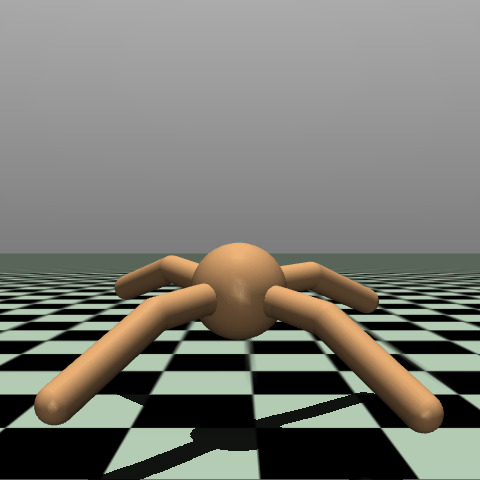
\includegraphics[width=0.3\linewidth]{assets/ant} &
    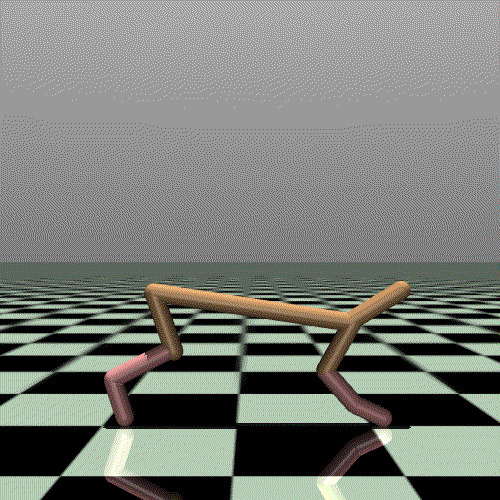
\includegraphics[width=0.3\linewidth]{assets/half_cheetah} \\
    (a) Ant & (b) Half Cheetah \\
    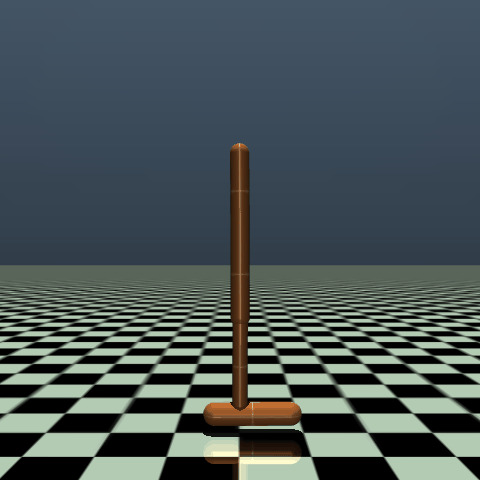
\includegraphics[width=0.3\linewidth]{assets/hopper} &
    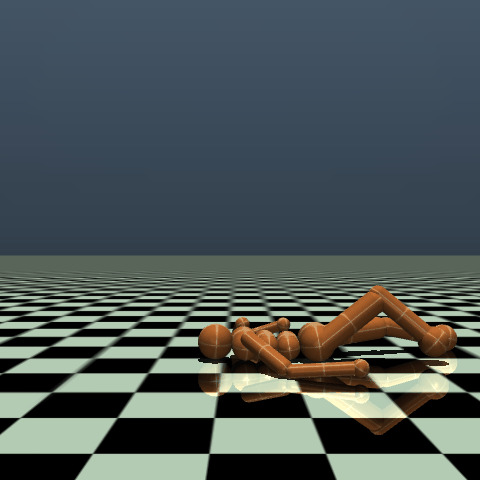
\includegraphics[width=0.3\linewidth]{assets/humanoid_standup} \\
    (c) Hopper & (d) Humanoid Standup \\
    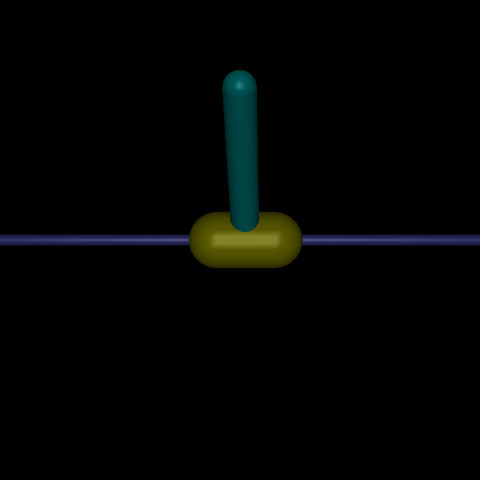
\includegraphics[width=0.3\linewidth]{assets/inverted_pendulum} &
    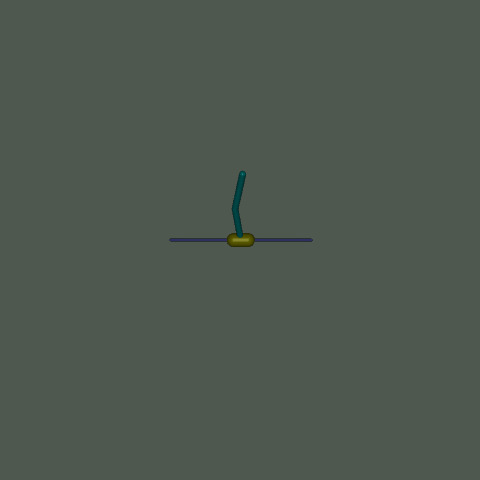
\includegraphics[width=0.3\linewidth]{assets/inverted_double_pendulum} \\
    (e) Inverted Pendulum & (f) Inverted Double Pendulum \\
  \end{tabular}
  \caption{MuJoCo Environments used in this work}
  \label{fig:mujoco_env}
  \Description{MuJoCo Environments used in this work}
\end{figure}

\subsection{Dynamic Memory}
Dynamic memory plays a crucial role in evolving program graphs, particularly 
in multi-task learning (MTL), by providing a flexible and adaptive
mechanism for encoding and processing temporal information. Unlike static memory 
architectures, which impose fixed storage structures, dynamic memory allows each 
program within an evolving graph to independently adjust its memory representation 
based on task demands. This adaptability facilitates more efficient learning and 
decision-making, ultimately accelerating evolutionary processes.

Dynamic memory within program graphs consists of three primary types:
\begin{itemize}
  \item \textbf{Scalar Memory}: Stores single numerical values, useful for tracking individual state variables.
  \item \textbf{Vector Memory}: Represents data as structured arrays, allowing operations across multiple related values.
  \item \textbf{Matrix Memory}: Enables higher-dimensional representations, which can encode richer state information 
  and facilitate more complex transformations.
\end{itemize}

Each program selects an appropriate memory type based on its computational needs, 
and mutations can modify both the type and dimensionality of the memory structures over the course of evolution.

\subsection{Tangled Program Graphs}
Tangled Program Graphs (TPG) is an RL framework developed by McMaster University’s Creative Algorithm Lab under the guidance of Dr. Stephen Kelly.
It leverages genetic programming principles to evolve agents capable of solving complex tasks in dynamic environments. Traditional RL methods,
such as deep reinforcement learning (DRL), often rely on neural networks that require significant computational resources and large datasets for training.
~\cite{Winkler2025}  In contrast, TPG uses genetic programming to evolve agents that can learn and adapt to their environment through a process of 
selection, mutation, and crossover. This unique approach allows TPG to achieve competitive performance in RL tasks with better computation
efficiency than DRL methods.~\cite{Winkler2025}

TPG revolves around the concept of emergent modularity, where agents are composed of interconnected programs that map environmental states to actions.
These programs are organized into hierarchical structures, known as program graphs, that allow agents to break complex tasks into simpler subtasks.~\cite{Kelly21} To incorporate TPG with multi-task learning, an agent will have to be trained to perform multiple tasks sequentially.
This is challenging as the agent must balance different objectives and environments while  avoiding catastrophic forgetting
(learning a new task causes agent to forget previously learned tasks, effectively wasting progress).~\cite{Kelly21} TPG’s
hierarchical and modular structure however, is able to tackle this challenge by allowing agents to dynamically adapt to different tasks by 
“recombining specialized behaviors”.~\cite{Kelly21} TPG has been previously used to evolve agents capable of solving six distinct RL benchmarks from OpenAI’s
Classic Control suite, including CartPole, Acrobot, and Pendulum.~\cite{Kelly21} Currently, TPG is being further developed to gauge it’s
capability of integrating multi-task learning with more complex MuJoCo environments.

\section{Motivation}
The primary motivation behind this research and development effort is to enhance the performance and efficiency of TPG in complex environments, specifically within the MuJoCo physics simulation framework. MuJoCo environments, such as Ant, Half Cheetah, and Humanoid Standup, present significant challenges due to their high-dimensional state and action spaces, as well as their dynamic nature. These environments require agents to learn proper control policies that generalize across diverse scenarios, making them ideal benchmarks for evaluating the scalability and adaptability of TPG.

The goal is to both improve performance and increase efficiency. Performance will be measured by the best fitness score achieved by the TPG agent, reflecting its ability to maximize cumulative rewards. Efficiency will be measured by the number of generations required for the agent to converge to an optimal state, which also reflects the time and computational resources needed for training. By integrating dynamic memory and optimizing the evolutionary process, this research aims to reduce the time to learn while maintaining or improving the quality of the learned policies.

\section{Research Questions}

Building on the motivation that memory mechanisms can significantly improve an agent's ability to handle temporal dependencies in reinforcement learning (RL)~\cite{Djavaherpour24}, we investigate the specific contribution of \textbf{dynamic memory} within the Tangled Program Graphs (TPG) framework. Prior work has shown that TPG agents without any persistent memory perform poorly on tasks requiring temporal integration (e.g., partially observable environments)\cite{Kelly21}, underscoring the need for effective memory strategies. While the standard TPG uses a fixed-size (static) memory for all tasks, a \textit{dynamic} memory approach---where the agent can allocate and manage memory on the fly---offers a theoretically more flexible alternative~\cite{Kelly21TELO}. Such dynamic memory could allow hierarchical RL agents to encode and retrieve information more adaptively over time~\cite{Kelly21TELO}. We therefore pose the following research questions, which align with our methodology and experiments on continuous control tasks (MuJoCo environments):

\begin{enumerate}
    \item \textbf{RQ1: Role in Single-Task Learning ---} \textit{How does the incorporation of dynamic memory influence learning performance in single-task MuJoCo control tasks using TPG, compared to a fixed-memory setup?} This question examines whether a TPG agent endowed with dynamic memory attains higher rewards or learns more efficiently on individual tasks (each trained in isolation) versus the baseline of fixed (static) memory. We seek to determine if dynamic memory provides any tangible benefit in single-task scenarios, or if fully observable single tasks already suffice with a static memory mechanism.

    \item \textbf{RQ2: Role in Multi-Task Learning \& Adaptability ---} \textit{Does dynamic memory improve an agent's adaptability and performance in multi-task learning scenarios within TPG?} In other words, when a single TPG agent must handle \textbf{multiple} MuJoCo tasks, does a dynamic memory mechanism enable better task identification, knowledge sharing, or policy adaptation across tasks compared to fixed memory? This question probes whether dynamic memory helps the hierarchical TPG agent adjust to different tasks (potentially with diverse state dynamics) more effectively. Prior studies suggest that memory is crucial for multi-task agents to approach the performance of task-specific agents~\cite{Kelly21}, so here we ask if allowing memory to be managed dynamically further enhances the agent's multi-task learning capability and resilience to task variations.

    \item \textbf{RQ3: Performance vs. Computational Efficiency ---} \textit{What are the effects of using dynamic memory on learning efficiency and computational cost in TPG, relative to a fixed-memory approach?} We compare dynamic and fixed memory configurations to assess trade-offs between \textbf{learning performance} (e.g., speed of convergence, final reward achieved) and \textbf{computational efficiency} (e.g., runtime or memory overhead). This question addresses whether any gains from dynamic memory come at the expense of significantly higher computational complexity. Ideally, an enhanced memory system should improve learning outcomes without incurring prohibitive overhead. For instance, recent work demonstrated that better memory management can boost performance while \textbf{preserving} computational efficiency~\cite{Djavaherpour24}. Here, we examine if a dynamic memory design achieves a similar balance in practice.

    \item \textbf{RQ4: Validation of Theoretical Benefits ---} \textit{Do our empirical findings validate the theoretical motivations for integrating dynamic memory into a hierarchical RL framework like TPG?} Dynamic memory is hypothesized to enable more effective temporal credit assignment and hierarchical problem decomposition~\cite{Kelly21TELO}. This question asks whether the introduction of dynamic memory in TPG indeed yields these anticipated benefits. Specifically, we investigate if the dynamic memory agent exhibits improved \textbf{temporal integration} of past information and a more flexible reallocation of memory resources that align with the problem's demands. By comparing the behaviors and structures emerging in dynamic-memory TPG agents versus static-memory ones, we aim to confirm whether dynamic memory provides the expected advantages (such as better handling of partial observability and long-term dependencies) in a real experimental setting.
\end{enumerate}

\section{Methodology}

This study evaluates task performance parameters such as generation time and 
fitness level through experiments conducted in their respective MuJoCo environments 
(see Figure~\ref{fig:mujoco_env}). The methodology follows a two-phase approach: establishing baselines
and integrating dynamic memory. We compare between baseline and dynamic memory-enhanced
experiments that were conducted using statistical plots and TPG-generated data. All
experiments utilized High Performance Parallel Compute (HPPC) resourcesprovided by the
Digital Research Alliance of Canada (“The Alliance”). Each experiment was run with three
random seeds for a three-hour duration.

\subsection{Baseline Experiments}
We conducted single-task and multi-task experiments using the following MuJoCo environments:
inverted pendulum, inverted double pendulum, and half-cheetah. Single-task experiments used standardized
hyperparameters listed in Table~\ref{tab:hyperparameters}. Each experiment was assigned a specific memory\_size 
parameter value basedon the dimensionality of the observation space, detailed in Table~\ref{tab:observation_space}.

\begin{table*}
  \caption{Hyperparameters for MuJoCo environments, single-task team population, and program population}\label{tab:hyperparameters}
  \centering
  \begin{tabular}{llcllcll}
    \toprule
    \multicolumn{2}{c}{\textbf{MuJoCo parameters}} & & \multicolumn{2}{c}{\textbf{Team population}} & & \multicolumn{2}{c}{\textbf{Program population}} \\
    \cmidrule(r){1-2} \cmidrule(lr){4-5} \cmidrule(l){7-8}
    \textbf{Parameter} & \textbf{Value} & & \textbf{Parameter} & \textbf{Value} & & \textbf{Parameter} & \textbf{Value} \\
    \midrule
    Max timestep & 1000 & & Agent (root team) population size & 1000 & & Initial program size & 10 \\
    Reward control weight & 0.5 & & Initial team size & 1 & & $p_\text{delete}$ & 0.2 \\
    Number of training evaluations & 20 & & Max team size & 10 & & $p_\text{add}$, $p_\text{swap}$, $p_\text{mutate}$ & 0.25 \\
    Number of test evaluations & 1 & & $n\_root\_gen$ & 100 & & $mem_\text{min}$ & 2 \\
    Number of validation evaluations & 0 & & & & & $mem_\text{max}$ & 32 \\
    & & & & & & $p_\text{mem}$ & 0.0 \\
    \bottomrule
  \end{tabular}
  \caption*{\small \textit{Note:} $n\_root\_gen$ denotes the number of new root teams to create each generation. $p_\text{x}$ in which $x \in \{add, delete, swap, mutate\}$ are the probabilities of adding, deleting, swapping, or mutating instructions within a program. $p_\text{mem}$ is the probability of changing the memory size, $mem_\text{size}$, within the $mem_\text{min}$ and $mem_\text{max}$ interval.}
\end{table*}

\begin{table}
  \caption{Observation and action space sizes for the considered problems~\cite{FaramaFoundation24}}\label{tab:observation_space}
  \begin{tabular}{lll}
    \toprule
    \textbf{Environment}&\textbf{Obs.}~$\mathcal{O}$&\textbf{Act.}~$\mathcal{A}$\\
    \midrule
    Inverted pendulum & $\mathbb{R}^4$ & [-3, -3]\\
    Inverted double pendulum & $\mathbb{R}^9$ & [-1, 1]\\
    Half cheetah & $\mathbb{R}^{17}$ & [-1, 1]\\
  \bottomrule
\end{tabular}
\end{table}

For multi-task experiments, we utilize the same MuJoCo environments. However, the root team size was increased to 3000,
and $n\_root\_gen$ was increased to 300 to accommodate the added complexity of multi-task learning. Two multi-task
experiments were conducted:

\begin{enumerate}
  \item \textbf{Two-environment multi-task:} Inverted pendulum and inverted double pendulum.
  \item \textbf{Three-environment multi-task:} Inverted pendulum, inverted double pendulum, and half cheetah.
\end{enumerate}

The initial $mem_\text{size}$ parameter was set to 4 for the two-environment multi-task experiment and 17 for the three-environment
multi-task experiment.

\subsection{Dynamic Memory Experiments}
To evaluate the benefits of adaptive memory allocation, we implemented a dynamic memory strategy by increasing the probability
of changing memory size, $p_\text{mem}$, to 10\% (0.1). The effects of this modification were assessed across the same baseline experiments.

\begin{itemize}
  \item For single-task experiments, the minimum and maximum values for $mem_\text{size}$ remained fixed at 2 and 32, respectively.
  \item For multi-task experiments, the minimum and maximum values for $mem_\text{size}$ were dynamically adjusted based on the smallest
  and largest observation space dimensions among the participating environments.
\end{itemize}

\subsection{Data Collection}
For each experiment, performance metrics were systematically recorded and extracted from the \texttt{.std} output files,
then parsed into structured \texttt{.csv} files. These \texttt{.csv} files were categorized into:

\begin{itemize}
  \item \textbf{Timing Metrics:} Measures of computational timing.
  \item \textbf{Selection Metrics:} Data on operations used, fitness level, and instruction count.
  \item \textbf{Replacement Metrics:} Statistics on team and program numbers.
  \item \textbf{Removal Metrics:} Information on program and team deletions.
\end{itemize}

Key performance indicators analyzed include:

\begin{itemize}
  \item \textbf{Best Fitness Score:} The highest fitness score achieved during execution.
  \item \textbf{Generations to Convergence:} The number of generations required to reach a specified performance threshold.
  \item \textbf{Effective Program Instructions:} The number of program instructions contributing to the final output.
\end{itemize}

After data collection, comparative analyses were conducted to evaluate the differences between baseline and dynamic memory configurations
across both single-task and multi-task experiments. Visualization techniques, including comparative plots, were used to identify performance
trends and assess the impact of dynamic memory integration.

\section{Baseline Experiments Results}
This section presents the performance outcomes of the baseline experiments conducted in 
the MuJoCo environments, including single-task and multi-task scenarios. The evaluation 
metrics focus on \textbf{Best Fitness Score} and \textbf{Effective Program Instruction Count}, as illustrated in 
Figures~\ref{fig:best_fitness} and~\ref{fig:effective_program}, respectively.

\subsection{Best Fitness Score Analysis}
The \textbf{Best Fitness Score} metric, depicted in Figure~\ref{fig:best_fitness}, provides insights into the overall 
learning progress of the different experiments. The results highlight several key observations:

\begin{itemize}
  \item \textbf{Single-task environments}: The fitness scores for Half Cheetah and Inverted Pendulum show that while both static and dynamic memory setups improve over time, dynamic memory consistently achieves higher fitness scores faster.
  \item \textbf{Multi-task environments}: Dynamic memory demonstrates a clear advantage, particularly in the Two- and Three-task multi-task setups. It outperforms static memory across generations, highlighting its ability to adapt more effectively to increasing task complexity.
\end{itemize}

\subsection{Program Instruction Count Analysis}
Figure~\ref{fig:effective_program} presents the results of the \textbf{Effective Program Instruction Count}, a key metric reflecting the number of active 
program instructions contributing to task performance.

\begin{itemize}
  \item \textbf{Single-task environments}: Dynamic environments show more fluctuations in active instruction counts, indicating frequent adaptation for optimization. In contrast, static environments stabilize early, limiting flexibility.
  \item \textbf{Multi-task environments}: The Effective Program Instruction Count is significantly higher in dynamic multi-task setups, suggesting better management of complex learning structures. Static environments struggle to scale efficiently.
\end{itemize}

% \afterpage{
%   \clearpage
  
  
%   \clearpage
% }
% \afterpage{
%   \clearpage


%   \clearpage
% }

\section{Results and Conclusion}

This research investigated the impact of dynamic memory within Tangled Program Graphs (TPG) for 
reinforcement learning in MuJoCo environments, addressing key questions regarding its role in 
STL, MTL, computational efficiency, and validation of theoretical benefits.

\subsection{RQ1: Role in Single-Task Learning} 
Our experiments in single-task MuJoCo control tasks (Half Cheetah, Inverted Pendulum) demonstrate 
that TPG agents with dynamic memory achieve higher fitness scores and faster learning convergence 
compared to those with fixed memory. This suggests that dynamic memory enhances the agent's ability 
to adapt to task-specific dynamics even in relatively simple, fully observable environments.

\subsection{RQ2: Role in Multi-Task Learning \& Adaptability} 
In multi-task learning scenarios (Two-Environment and Three-Environment setups), dynamic memory exhibited a clear advantage. 
Agents with dynamic memory showed significantly improved adaptability and performance, achieving 
higher fitness scores across generations compared to their fixed-memory counterparts. This indicates 
that dynamic memory facilitates better task identification, knowledge sharing, and policy adaptation 
across multiple tasks with varying state dynamics.

\subsection{RQ3: Performance vs. Computational Efficiency}
The results indicate that the performance gains achieved through dynamic memory do not come at a 
prohibitive computational cost. While dynamic memory agents demonstrate more fluctuations in active 
program instruction counts, indicating frequent adaptation, the overall learning efficiency, as measured 
by generations to convergence and best fitness score, is enhanced. This suggests that dynamic memory 
allows for more effective utilization of computational resources, leading to improved learning outcomes without significant overhead.

\subsection{RQ4: Validation of Theoretical Benefits}
Our empirical findings largely validate the theoretical motivations 
for integrating dynamic memory into TPG. The improved performance in both single-task and multi-task scenarios supports 
the hypothesis that dynamic memory enables more effective temporal credit assignment and hierarchical problem decomposition. 
The dynamic memory agents exhibited a more flexible reallocation of memory resources, aligning with the problem's demands 
and demonstrating the anticipated benefits of better handling partial observability and long-term dependencies.

In conclusion, this research provides strong evidence for the benefits of dynamic memory within TPG for reinforcement 
learning in complex MuJoCo environments. The ability to adaptively allocate memory based on task demands enhances both 
learning performance and efficiency, particularly in multi-task scenarios. These findings highlight the potential of 
dynamic memory as a key component in developing more robust and adaptable RL agents capable of tackling real-world challenges. 
Future work should focus on further optimizing the dynamic memory allocation process and exploring its application 
in even more complex and partially observable environments.

%%
%% The acknowledgments section is defined using the "acks" environment
%% (and NOT an unnumbered section). This ensures the proper
%% identification of the section in the article metadata, and the
%% consistent spelling of the heading.
\begin{acks}
To Dr. Stephen Kelly, for guiding us throughout the research process and providing valuable insights and feedback.
\end{acks}

%%
%% The next two lines define the bibliography style to be used, and
%% the bibliography file.
\bibliographystyle{assets/ACM-Reference-Format}
\bibliography{assets/research-base}
\clearpage
\appendix

\onecolumn
\begin{figure*}
  \section{Additional Figures}
  \subsection{Best Fitness Score Results}
  \centering
  \scalebox{0.87}{
  \begin{tabular}{p{1\linewidth}}
    \begin{overpic}[clip, trim=25 25 125 0, width=0.5\textwidth]{assets/pdf/static/best_fitness/half_cheetah.pdf}
      \put(160,20){\color{black!50}Static Half Cheetah} % Adjust position
      \put(-15,50){\rotatebox{90}{\color{black}\LARGE Best Fitness}} % Adjust position and size
    \end{overpic}
    \begin{overpic}[clip, trim=25 25 125 0, width=0.5\textwidth]{assets/pdf/dynamic/best_fitness/half_cheetah.pdf}
      \put(145,20){\color{black!50}Dynamic Half Cheetah} % Adjust position
    \end{overpic}
  \end{tabular}
  }

  \scalebox{0.87}{
  \begin{tabular}{p{1\linewidth}}
    \begin{overpic}[clip, trim=25 25 125 0, width=0.5\textwidth]{assets/pdf/static/best_fitness/ip.pdf}
      \put(160,20){\color{black!50}\shortstack[r]{Static \\ Inverted Pendulum}} % Adjust position
      \put(-15,50){\rotatebox{90}{\color{black}\LARGE Best Fitness}} % Adjust position and size
    \end{overpic}
    \begin{overpic}[clip, trim=25 25 125 0, width=0.5\textwidth]{assets/pdf/dynamic/best_fitness/ip.pdf}
      \put(160,20){\color{black!50}\shortstack[r]{Dynamic \\ Inverted Pendulum}} % Adjust position
    \end{overpic}
  \end{tabular}
  }

  \scalebox{0.87}{
  \begin{tabular}{p{1\linewidth}}
    \begin{overpic}[clip, trim=25 25 125 0, width=0.5\textwidth]{assets/pdf/static/best_fitness/multitask_general.pdf}
      \put(130,20){\color{black!50}\shortstack[r]{Static \\ Two-Environment Multi-task}} % Adjust position
      \put(-15,50){\rotatebox{90}{\color{black}\LARGE Best Fitness}} % Adjust position and size
    \end{overpic}
    \begin{overpic}[clip, trim=25 25 125 0, width=0.5\textwidth]{assets/pdf/dynamic/best_fitness/multitask_general.pdf}
      \put(125,20){\color{black!50}\shortstack[r]{Dynamic \\ Two-Environment Multi-task}} % Adjust position
    \end{overpic}
  \end{tabular}
  }

  \scalebox{0.87}{
  \begin{tabular}{p{1\linewidth}}
    \begin{overpic}[clip, trim=25 25 125 0, width=0.5\textwidth]{assets/pdf/static/best_fitness/multitask_hc.pdf}
      \put(125,20){\color{black!50}\shortstack[r]{Static \\ Three-Environment Multi-task}} % Adjust position
      \put(-15,50){\rotatebox{90}{\color{black}\LARGE Best Fitness}} % Adjust position and size
    \end{overpic}
    \begin{overpic}[clip, trim=25 25 125 0, width=0.5\textwidth]{assets/pdf/dynamic/best_fitness/multitask_hc.pdf}
      \put(120,20){\color{black!50}\shortstack[r]{Dynamic \\ Three-Environment Multi-task}} % Adjust position
    \end{overpic}
  \end{tabular}
  }
  
  \caption{Best Fitness Score results from Single and Multi-task Baseline Experiments}
  \label{fig:best_fitness}
\end{figure*}
\clearpage
\begin{figure*}
  \subsection{Effective Program Instruction Count Results}

  \centering
  \scalebox{0.87}{
  \begin{tabular}{p{1\linewidth}}
    \begin{overpic}[clip, trim=25 25 125 0, width=0.5\textwidth]{assets/pdf/static/effective_program_instruction_count/half_cheetah.pdf}
      \put(160,20){\color{black!50}Static Half Cheetah} % Adjust position
      \put(-15,20){\rotatebox{90}{\color{black}\LARGE Effective Instruction Count}} % Adjust position and size
    \end{overpic}
    \begin{overpic}[clip, trim=25 25 125 0, width=0.5\textwidth]{assets/pdf/dynamic/effective_program_instruction_count/half_cheetah.pdf}
      \put(145,20){\color{black!50}Dynamic Half Cheetah} % Adjust position
    \end{overpic}
  \end{tabular}
  }

  \scalebox{0.87}{
  \begin{tabular}{p{1\linewidth}}
    \begin{overpic}[clip, trim=25 25 125 0, width=0.5\textwidth]{assets/pdf/static/effective_program_instruction_count/ip.pdf}
      \put(160,20){\color{black!50}\shortstack[r]{Static \\ Inverted Pendulum}} % Adjust position
      \put(-15,20){\rotatebox{90}{\color{black}\LARGE Effective Instruction Count}} % Adjust position and size
    \end{overpic}
    \begin{overpic}[clip, trim=25 25 125 0, width=0.5\textwidth]{assets/pdf/dynamic/effective_program_instruction_count/ip.pdf}
      \put(160,20){\color{black!50}\shortstack[r]{Dynamic \\ Inverted Pendulum}} % Adjust position
    \end{overpic}
  \end{tabular}
  }

  \scalebox{0.87}{
  \begin{tabular}{p{1\linewidth}}
    \begin{overpic}[clip, trim=25 25 125 0, width=0.5\textwidth]{assets/pdf/static/effective_program_instruction_count/multitask_general.pdf}
      \put(130,20){\color{black!50}\shortstack[r]{Static \\ Two-Environment Multi-task}} % Adjust position
      \put(-15,20){\rotatebox{90}{\color{black}\LARGE Effective Instruction Count}} % Adjust position and size
    \end{overpic}
    \begin{overpic}[clip, trim=25 25 125 0, width=0.5\textwidth]{assets/pdf/dynamic/effective_program_instruction_count/multitask_general.pdf}
      \put(125,20){\color{black!50}\shortstack[r]{Dynamic \\ Two-Environment Multi-task}} % Adjust position
    \end{overpic}
  \end{tabular}
  }

  \scalebox{0.87}{
  \begin{tabular}{p{1\linewidth}}
    \begin{overpic}[clip, trim=25 25 125 0, width=0.5\textwidth]{assets/pdf/static/effective_program_instruction_count/multitask_hc.pdf}
      \put(125,20){\color{black!50}\shortstack[r]{Static \\ Three-Environment Multi-task}} % Adjust position
      \put(-15,20){\rotatebox{90}{\color{black}\LARGE Effective Instruction Count}} % Adjust position and size
    \end{overpic}
    \begin{overpic}[clip, trim=25 25 125 0, width=0.5\textwidth]{assets/pdf/dynamic/effective_program_instruction_count/multitask_hc.pdf}
      \put(120,20){\color{black!50}\shortstack[r]{Dynamic \\ Three-Environment Multitask}} % Adjust position
    \end{overpic}
  \end{tabular}
  }
  
  \caption{Effective Program Instruction Count results from Single and Multi-task Baseline Experiments}\label{fig:effective_program}
\end{figure*}
\twocolumn

%%
%% If your work has an appendix, this is the place to put it.
% \appendix

\end{document}
\endinput
%%
%% End of file `ResearchReport.tex'.
